\chapter{Synchronous Message Exchange}

In the previous chapter we went through the theory behind logic design, all the way from the introduction of Boolean algebra to gate-level implementation of logic units. We will in this chapter use those ideas to implement logic units in synchronous message exchange (SME). This will serve as a means to introduce SME to the reader and further cement former logic design ideas.

Starting out we will go through a short introduction behind the inspiration for SME, Communicating Sequential Processes. Hereafter we will go through the theory and syntax of SME with an emphasis on real examples, as i believe this is the most efficient manner of introducing SME to the reader.  

\section{Communicating Sequential Processes} \change{Rewrite this section} \improvement{add examples of a process and channels}
    
    When working with multiprocessor workloads one will quickly realize the inconvenience of memory sharing. The non-determinism of having multiple processes reading and writing the same memory often results in unexpected behavior.
    
    A classic example of non-determinism would be the act of printing out the numbers one through ten, to your console using more than one thread. If the aforementioned code is executed multiple times, you will notice that the order of numbers would vary between the runs. This is due to the scheduler of the operating system, which one does not have control over. That can create race conditions (meaning the behavior in your code is dependent on the timing of different threads), which can cause unpredictable behavior and therefore bugs, which is undesirable.
    
    Various attempts has been made to solve this problem, such as the introduction of mutexes or locks. Though it does not solve our problem completely as these "solutions" introduces deadlocks, which is a state, where multiple processes are waiting for each other and the program stalls indefinitely. These deadlocks might not happen every run and thus introduces another layer of difficulty, as error reproducibility is essential for code debugging and therefore makes it hard to make reliable software.
    
    Communicating Sequential Processes (CSP) is an algebra first proposed by \citet{HoareC1978Csp} to solve exactly these issues.
    CSP is build on two very basic primitives one is the process (which should not be confused with operating system processes). A process could be an ordered sequence of operations. These processes do not share any memory, therefore one process cannot access a specific value in another process (which solves the problems we had with shared memory).
    
    The other primitive is channels, which is the way the processes communicate with each other. You can pass whatever you want through these channels, but once you pass the value, the process lose access to it. There are a lot of ways the processes and channels can be arranged. The most simple one can be found in figure \ref{fig:one_to_one}, which illustrates process 1 passing a value onto a channel which process 2 takes as input. Some different configurations can be found in figures  \ref{fig:one_to_many}-\ref{fig:many_to_many}. 
    
    Using these primitives as ones programming paradigm one can design multiprocess workloads without the shared memory problems mentioned earlier. The asynchronous nature of CSP will though be a problem for hardware models, as we will see shortly and is the fundamental inspiration behind synchronous message exchange. 

    \begin{figure}[h!]
        \hspace*{-1.25cm}
        \begin{subfigure}[t]{0.5\textwidth}
            \centering
            \subimport{tikz_stuff/}{one_to_one}
            \caption{CSP one to one}
            \label{fig:one_to_one}
        \end{subfigure}%
        \hspace*{1cm}
        \begin{subfigure}[t]{0.5\textwidth}
            \centering
            \subimport{tikz_stuff/}{one_to_many}
            \caption{CSP one to many}
            \label{fig:one_to_many}
        \end{subfigure}
        \vspace*{2cm}
        
        \hspace*{-1cm}
        \begin{subfigure}[b]{0.5\textwidth}
            \centering
            \subimport{tikz_stuff/}{many_to_one}
            \caption{CSP many to one}
            \label{fig:many_to_one}
        \end{subfigure}%
        \hspace*{1cm}
        \begin{subfigure}[b]{0.5\textwidth}
            \centering
            \subimport{tikz_stuff/}{many_to_many}
            \caption{CSP many to many}
            \label{fig:many_to_many}
        \end{subfigure}%
    \end{figure}
    
\section{Synchronous Message Exchange}
    The idea of using CSP for hardware modeling was first introduced in \citet{BPUSimulator2013} and later further developed in \cite{PyCSPFPGA}, where two students successfully implemented a vector processor using PyCSP (a CSP library for python).\improvement{ask where the idea to use csp for hardware came from}  They however found a number of shortcomings of using PyCSP for hardware modeling. The need for global synchronicity, when simulating hardware models using CSP, meant that additional channels were needed to simulate clock progress and emulation of latches among others. This caused an explosion of required channels and an unnecessary increase in complexity.
    
    They did however find that building isolated processes and then connecting them via channels proved to be a powerful approach for building larger hardware models. As in the unit testing method one can develop and test individual processes to then connecting them together and form larger hardware models.
    
    With this in mind a more suitable message-passing framework for hardware modeling was developed, with the following requirements:
    
    \begin{itemize}
        \item Globally synchronous
        \item Broadcasting channels
        \item Shared nothing
        \item Implicit latches
    \end{itemize} 
    
    all these observations laid the foundation behind synchronous message exchange (SME),  \citet{vinter2014synchronous}. 
    Since then the SME framework has been implemented in the .Net framework, \citet{skovhede2016building}, which is the version of SME that will be used throughout this thesis.
    
    We will not dwell further into the theory behind SME in this thesis. Instead we will be developing actual units in SME, that will be needed when we later implement the RISC-V architecture. The SME syntax will be introduced as we go through the examples and is intended to be a from-scratch introduction for the uninitiated reader. 

    \subsection{SME setup and structure}
        We will in this section go through the code structure I have decided to use for the development of all logic units. Much thought has been given to this and from previous experience doing code projects I would say it is good practice to think about the general structure of ones project for ease of development and future extensions.
        
        A modular design is essential as many logic units is going to be needed when implementing the RISC-V architecture. This also allows for easy debugging and testing, as individual units can be addressed before integrating them into a larger system. Each logic unit will also be separated into two files. One which contains all the buses and one which contains the function of the unit. The thought behind this is to help compartmentalize bus declarations from unit function and hopefully ease development.  
        
        In the following it is a prerequisite that .Net Core SDK\footnote{The SDK can be found here \url{https://dotnet.microsoft.com/download}} is installed on their respective systems to be able to run the code. All following code examples can be found by clicking \href{https://github.com/DanielRamyar/Master_Thesis/tree/master/SME_Implementations}{here} or if reading printed version the full link can be found in this footnote\footnote{\url{https://github.com/DanielRamyar/Master_Thesis/tree/master/SME_Implementations}}.
        
        In the following it should be noted that the equivalent to a channel in CSP, is a bus in SME. Buses however, are able to contain multiple signals/channels.  
        
        \subsubsection{Project structure example}
        We are going to build an AND gate for this example and will be the only section were the complete code is shown, as this section is meant to serve as a "quick start guide" for readers beginning their journey into SME. Subsequent sections will only show relevant parts of the code. 
        
        For this quick example we are going to start a project in a folder called .../ANDGate/, which is where all shown files are going to be placed.
        To do this we are going to open up a terminal window and navigate to the desired folder destination (for example the Desktop) and invoke the command: 
        
        \begin{lstlisting}[language=bash]
$ dotnet new console -n ANDGate
        \end{lstlisting}
        where "ANDGate" can be changed to a name of choice.
        
        Next navigate into the folder
        \begin{lstlisting}[language=bash]
$ cd ANDGate 
        \end{lstlisting}
        and add the necessary SME libraries
        \begin{lstlisting}[language=bash]
$ dotnet add package SME --version=0.4.0-beta
$ dotnet add package SME.GraphViz --version=0.4.0-beta
$ dotnet add package SME.Tracer --version=0.4.0-beta
$ dotnet add package SME.VHDL --version=0.4.0-beta
        \end{lstlisting}
        
        There should now exist 3 items inside the ANDGate folder: Program.cs, ANDGate.csproj and a folder called obj. If all went well we should now be able to begin with our project.
        
        I always find drawing a quick flowchart before implementing code gives a nice overview ones project. So in the spirit of this I've drawn out a quick sketch of the project in Figure \ref{fig:ANDGateSME}, which shows the two processes we are going to create, namely the SME simulator and the AND gate process.
        
        \begin{figure}[h!]
            \centering
            \subimport{tikz_stuff/}{ANDGateSME}
            \caption{Flowchart of AND gate SME project. Here the rectangles represent individual processes, which lies in a file of its own. The solid arrow represents a bus and dashed arrow a bus going to a clocked process.}
            \label{fig:ANDGateSME}
        \end{figure}  
        
        
\newpage
        Opening up the Program.cs file, we are going to add a couple of lines, as shown in Listing \ref{projectfile}. The Program.cs contains the Main() method of the project and is the entry point of any C\scalerel*{\#}{X} program. To use the SME library we import it with the "using SME" command as shown in the second line. 
        
        Within the Main() method, the first function we meet is the using function, this is just to ensure the resources is properly cleaned up after the simulation.
        
        Hereafter we see the simulation object, which as the name implies, is responsible for the simulation of the logic unit. We then pass the simulated input to the ANDgate object, which will then perform the AND operation (it is not necessary to pass the simulation object itself to the ANDGate, but is shown here to not cause confusion about how the simulation passes input values to the AND process). We will see how these objects are defined shortly. 
        
        Lastly we can configure the simulator object, which uses fluent syntax. In this case we configured it to build a CSV file, which shows what each bus contained at every clock cycle. We build a graph, which outputs a .dot file that shows how all the processes are connected and we transpile the code to VHDL. It should be noted that Run() should always be the last method called.
        
        The file which contains the Main() will ways be named project.cs in this thesis, but the naming is irrelevant.
        
        
        \lstinputlisting[language={[Sharp]C}, caption={The Program.cs file, which contains the Main() method for the project.},captionpos=b, label = projectfile]{/Users/danielramyar/Desktop/Thesis/SME_Implementations/ANDGate/Project.cs}  

        We are going to need a way to test our AND gate, this is what the simulation file is for and is shown in Listing \ref{simulatorfile}. Remember to name your namespace the same as in the project file. The first two definitions inside the simulation process creates or loads the two buses for the test. Notice that the gate output is labeled as an input bus and vice versa for the gate input. This is due to the simulation is a process in and of itself and therefore needs to output the test values to a bus, which the ANDGate process takes in as input.
        
        Now everything within the Run() method is what is going to be simulated and each time we want a new clock cycle to occur, we use the line \textit{await ClockAsync()}. In a simulation process any .Net library is allowed and is not going to get transpiled to a VHDL file. Therefore we can print the output of the AND gate to console to see whether or not it works correctly. We do this by transmitting data via the input bus, which contains two signals, in1 and in2. We then set the two signals to false wait a clock cycle and print the output. Since this is a fairly small system we can test for all input combinations and look at the outputs to see if the gate is behaving correctly. 

\begin{lstlisting}[language={[Sharp]C}, caption={The simulator file, which specifies how the simulation is run. Most lines in the run method are concatenated brievity.},captionpos=b, label = simulatorfile]
using System;
using SME;

namespace ANDGate {
    public class ANDGateSimulator : SimulationProcess {
        [InputBus]
        public readonly GateOutput output = Scope.CreateOrLoadBus<GateOutput>();
        
        [OutputBus]
        public readonly GateInputs input = Scope.CreateOrLoadBus<GateInputs>();
        
        public async override System.Threading.Tasks.Task Run() {
            Console.WriteLine("Starting test!\n");
            await ClockAsync();
            
            input.in_1 = false;
            input.in_2 = false;
            
            await ClockAsync();
            Console.WriteLine($"Gate input: {input.in_1} (Input 1) - {input.in_2} (Input 2)\n");
            Console.WriteLine($"AND gate output: {output.out_AND}");
            ...
            Console.WriteLine("Done testing!");
        }
    }
}
\end{lstlisting}

        Hereafter we are going to make our bus declarations in a new file called buses.cs. Looking at Listing \ref{busdeclarations}, we see that the bus declarations are made using the interface command, which inherits its fields and methods from the IBus interface. The name for the bus is free of choice and in this case are called GateInputs and GateOuputs respectively.
        
        A bus can contain multiple signals of various types. Since the AND gate evaluates binary values, the bool type has been chosen for the input and output signals. You may have noticed that all the signals have the InitialValue attribute. What this does is that once the bus is created it will contain an initial value. If this is not done one have to be careful not to read the bus before any value has been given to it, as this will crash the program.
        
        Hereafter we have the TopLevelInputBus and TopLevelOuputBus attributes, they tell SME which buses goes in and out of the hardware implementation. Remember that this attribute is only given to buses which interfacing with some outside process, in this case the simulation process. Internal buses should not be given this attribute. By a internal bus we mean a bus which is connecting processes inside the hardware implementation (see Figure \ref{fig:2BitDecoderSME} here the internal buses goes from the NOT gates to the AND gates) \note{finish this section}

        \lstinputlisting[language={[Sharp]C}, caption={The file where all bus declarations are made.},captionpos=b, label = busdeclarations]{/Users/danielramyar/Desktop/Thesis/SME_Implementations/ANDGate/Buses.cs}
        
        Lastly we are going to define our AND gate in a process class. We create a file called ANDGate.cs, where our process is going to lie. We see how the process is defined in Listing \ref{ANDGateProcess}. In line 5 we define the class ANDGate and since the AND gate is only going to execute once per cycle, we are going to inherit from the SimpleProcess class.
        
        We are then loading our output bus in lines 6-7 and declaring our input bus in lines 9-10. Then I have added a constructor, which checks whether or not the object passed from the simulator object (remember that we passed the simulator inputs in the project file) contains any values.
        
        Finally we have the OnTick method, which contains the logic that has to be performed. In line 16 we perform the logical AND operation between the two input signals and then passing it on to the output. The Ontick method makes sure that the code within runs exactly once per cycle.
        
        \lstinputlisting[language={[Sharp]C}, caption={This is where we define the function of the AND gate process.},captionpos=b, label = ANDGateProcess]{/Users/danielramyar/Desktop/Thesis/SME_Implementations/ANDGate/ANDgate.cs}
        
        Finally one run the project by returning to the terminal. In the directory where the project is placed one simply writes following command
        
        \begin{lstlisting}[language=bash]
$ dotnet run
        \end{lstlisting}
        this will output 3 files to a folder named output placed in the same directory as the project. These files consist of network.dot, trace.csv and a VHDL folder. The network.dot file is a graphical representation of our model, which we have shown in Figure \ref{fig:ANDGateDOTFile}. Next we have the trace.csv file, which shows what each signal in all buses contained at each clock cycle. This is a very helpful tool when debugging, as one can quickly identify problems if wrong values are spotted throughout the simulation.
        
        Lastly we the transpiled VHDL files in the VHDL folder, which we can verify using any VHDL simulator (GHDL is recommended). The folder contains a makefile, which automates this process, so you simply navigate to the VHDL folder in your terminal and run the command
        \begin{lstlisting}[language=bash]
        $ dotnet make
        \end{lstlisting}
        assuming that you have already installed GHDL on your system.
        
        \begin{figure}[h!]
                \centering
                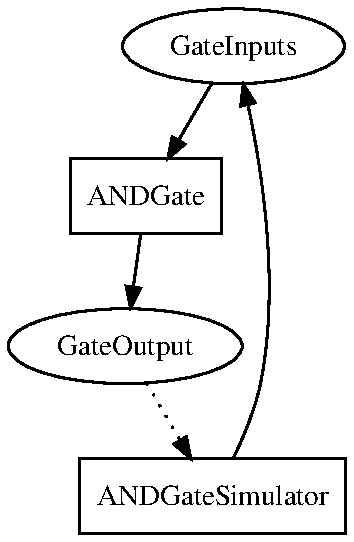
\includegraphics{pictures/ANDGate.pdf}
                \caption{Graphical representation of the AND gate generated by the outputted network.dot file. Here rectangles represent processes and ellipses buses. The arrows show the direction of the data flow, where a dotted line indicates data flow to a clocked process, which means that the process is activated on a rising clock edge.}
                \label{fig:ANDGateDOTFile}
            
        \end{figure} 
    
    \subsection{The Decoder}
        In this section we will start by implementing the 2-bit decoder (see \ref{section:Decoder}). First we set up the logic table, as shown in Table \ref{LogicTable:2BitDecoder}. We then derive the logic equation from the table: 
        
        \begin{equation}
        \label{Eq:2Bitdecoder}
            output = \overline{In1} \cdot \overline{In0} + \overline{In1} \cdot In0 + In1 \cdot \overline{In0} + In1 \cdot In0
        \end{equation}
        
        We notice from Eq. \ref{Eq:2Bitdecoder} that we need two NOT gates, four AND gates and four outputs. Since we only have 1 minterm per output no OR gates are necessary.
        We can then create a circuit diagram of the decoder, as shown in Figure \ref{fig:2BitDecoderSchematic} and use it as our design guide when we implement it in SME.
         
        
        \begin{table}[h!]
            \centering
            \begin{tabular}{|c|c||c|c|c|c|}
                \hline
                \multicolumn{2}{|c||}{\textbf{Input}}& \multicolumn{4}{c|}{\textbf{Output}}                  \\ \hline
                In1        & In0        & Out3 & Out2 & Out1 & Out0 \\ \hline
                0          & 0          & 0    & 0    & 0    & 1    \\ \hline
                0          & 1          & 0    & 0    & 1    & 0    \\ \hline
                1          & 0          & 0    & 1    & 0    & 0    \\ \hline
                1          & 1          & 1    & 0    & 0    & 0    \\ \hline
            \end{tabular}
            \caption{Logic Table of a 2 input decoder, where the binary representation of the input determines which output gets asserted. For example when In1=1, In0=0 output 1 will get asserted as the binary representation for 2 is 10.}
            \label{LogicTable:2BitDecoder}
        \end{table}
    
        \begin{figure}[h!]
            \centering
            \subimport{tikz_stuff/}{2BitDecoderSchematic}
            \caption{Flowchart of AND gate SME project. Here the rectangles represent individual processes, which lies in a file of its own. The solid arrow represents a bus and dashed arrow a bus going to a clocked process.}
            \label{fig:2BitDecoderSchematic}
        \end{figure}
    
        \begin{figure}[h!]
            \centering
            \subimport{tikz_stuff/}{2BitDecoderSME}
            \caption{Flowchart of decoder SME project. Here the rectangles represent individual processes. The solid arrow represents a bus and the dashed arrow a bus going to a clocked process. Solid dots show extension of the same bus and any crossing lines are not connected}
            \label{fig:2BitDecoderSME}
        \end{figure}    
        



    
    
